\documentclass[11pt,a4paper]{report}
%
% $Id: main.tex,v 1.1 2002-03-14 10:43:41 jabril Exp $
%
%2345678901234567890123456789012345678901234567890123456789012345678901234567890
%        1         2         3         4         5         6         7         8
%
\usepackage[a4paper,offset={0pt,0pt},hmargin={2cm,2cm},vmargin={1cm,1cm}]{geometry}
\usepackage[catalan]{babel}
\usepackage{graphics}
\usepackage[dvips]{graphicx}
%% pstricks
\usepackage[dvips]{pstcol}
\usepackage{pstricks}
%\usepackage{pst-node}
%\usepackage{pst-char}
%\usepackage{pst-grad}
%% bibliography
\usepackage{natbib}
%% latex2html
\usepackage{url}
\usepackage{html}     
\usepackage{htmllist} 
%% tables    
\usepackage{dcolumn}
%\usepackage{colortbl}
%\usepackage{multirow}
%\usepackage{hhline}
%\usepackage{tabularx}
%% seminar
%\usepackage{semcolor,semlayer,semrot,semhelv,sem-page,slidesec}
%% draft watermark
%\usepackage[all,dvips]{draftcopy}
%\draftcopySetGrey{0.9}
%\draftcopyName{CONFIDENTIAL}{100}
%% layout
\usepackage{fancyhdr} % Do not use \usepackage{fancybox} -> TOCs disappear
%\usepackage{lscape}
%\usepackage{rotating}
%\usepackage{multicol}
%\usepackage{version}
%% fonts
\usepackage{times}\fontfamily{ptm}\selectfont
\usepackage{t1enc}

\input ColorDefs.tex %%%%% Colors for gff2ps
\input defs.tex      %%%%% Common Definitions File

%%%%% Setting text for footers and headers
\fancyhead{} % clear all fields
\fancyfoot{} % clear all fields
\fancyhead[RO,LE]{\thepage}
\fancyhead[LO,RE]{\shorttit\quad\rightmark}
\fancyfoot[LO,LE]{\small\textbf{\genomelab}}
\fancyfoot[CO,CE]{\small\textsl{\authorshort}}
\fancyfoot[RO,RE]{\small\textbf{\today}}
\renewcommand{\headrulewidth}{1pt}
\renewcommand{\footrulewidth}{1pt}
%%%%%
\usepackage{fancyvrb}
\newcommand{\versioncontrol}{
\begin{center}
\begin{minipage}[c]{50ex}
\VerbatimInput[fontfamily=courier,
               fontsize=\small,fontseries=b]{DEA.tex}
\end{minipage}
\end{center}
}

%%%%%%%%%%%%%%%%%%%%%%%%%%%%%%%%%%%%%%%%%%%%%%%%%%%%%%%
\includeonly{
   title,
   tocs,
   thanks,
   intro,
   matimet,
   results,
   tools,
   papers
}
%%%%%%%%%%%%%%%%%%%%%%%%%%%%%%%%%%%%%%%%%%%%%%%%%%%%%%%
\begin{document}

%
% $Id: title.tex,v 1.3 2002-03-11 18:25:37 jabril Exp $
%
\pagestyle{empty}

\begin{titlepage}

\ \vfill
\begin{center}
\textbf{\Huge \tit}\\[5ex]

% \textbf{\Large Authors List Here}\\[1ex]
\textbf{\Large Josep F. Abril}\\[1ex]
\textbf{\Large Gen\'{\i}s Parra}\\[1ex]
\textbf{\Large Roderic Guig\'o}\\[5ex] % \raisebox{0.85ex}{\footnotesize$\,\dag$}\\[0.5ex]

\textbf{\large --- \today ---}\\[10ex]

\vfill

\begin{raggedleft}
\showaffiliation
\raisebox{0.85ex}{\footnotesize$\dag\,$}{\large e-mail: {\mtjabril}, {\mtgparra} and {\mtrguigo}}\\
\end{raggedleft}
\end{center}

\end{titlepage} %'

\ \vfill
\versioncontrol

\newpage

\begin{abstract}
\begin{center}
\parbox{0.75\linewidth}{
\progdesc
} % parbox
\end{center}
\end{abstract}

\newpage

\vfill
\begin{raggedleft}
A la paci�ncia de les dones, en especial de la meva\ldots
\end{raggedleft}
\vfill

\newpage % EMPTY PAGE


\newpage %%%%%%%%%%%%%%%%%%%% FRONTMATTER

%
% $Id: tocs.tex,v 1.1 2002-03-11 11:44:55 jabril Exp $
%
\pagenumbering{roman}
\setcounter{page}{1}
\pagestyle{fancy}
% Marks redefinition must go here because pagestyle 
% resets the values to the default ones.
\renewcommand{\sectionmark}[1]{\markboth{}{\thesection.\ #1}}
\renewcommand{\subsectionmark}[1]{\markboth{}{\thesubsection.\ \textsl{#1}}}

\tableofcontents
\listoftables
\listoffigures

\vfill
\begin{center}
{\small$<$ \verb$Id: tocs.tex,v 1.1 2002-03-11 11:44:55 jabril Exp $$>$ }
\end{center}


%
% $Id: thanks.tex,v 1.2 2002-03-13 10:14:20 jabril Exp $
%
%2345678901234567890123456789012345678901234567890123456789012345678901234567890
%        1         2         3         4         5         6         7         8
%
\chapter*{Agra�ments}
\addcontentsline{toc}{chapter}{Agra�ments}

% To my wife...
gff2ps -> Montse Barbany (CSIC), users [especially Martin Reese, Celera genome annotaation team, ...]
aplot -> Thomas Wiehe and Steffi Gebauer-Jung, Mathias Platzer - Gernot Gl�eckner - Karol Szafransky - ??? and the people at IMB-Jena.
geneid -> Enrique Blanco, ...
sgp -> Mouse Genome Consortium, Michael Brent, Jim Kent ...
sysadmin -> Xavi Fustero per la seva paci�ncia tenint cura de les actualitzacions constants de les bases de dades de seq��ncies i per haver de treballar amb uns usuaris sovint for�a exigents.
internet -> google, perl -> Larry Wall, GNU per tot el sofware de qualitat i de domini p�blic disponible.


\newpage %%%%%%%%%%%%%%%%%%%% MAINMATTER
\pagenumbering{arabic}
\setcounter{page}{1}

%
% $Id: intro.tex,v 1.3 2002-03-13 23:53:10 jabril Exp $
%
%2345678901234567890123456789012345678901234567890123456789012345678901234567890
%        1         2         3         4         5         6         7         8
%
\chap{Introducci�}

\sctn{Aspectes Biol�gics.}

\subsctn{Les seq��ncies gen�miques.}

Entre finals del 1989 i principis del 1990 es van definir les bases del que m�s tard s'anomenaria el Projecte Genoma Hum�, que consistiria en obtenir la seq��ncia de nucle�tids que composen les mol�cules de DNA de la nostra esp�cie.
Gr�cies a les noves tecnologies, que han perm�s automatitzar els processos tant al laboratori com en l'an�lisi, en els darrers anys hem pogut assistir a l'explossi� exponencial de les dades gen�miques sobre seq��cies de diferents esp�cies (veieu la taula~\ref{tbl:seqdgenomes}). Aix� no hauria estat possible sense l'ajut de les m�quines seq�enciadores i del m�tode de seq�enciaci� per \textit{shotgunn}, per� tampoc sense els aven�os a nivell de computaci� que han vingut de la m� de la Bioinform�tica.

\begin{table}[!b] %%%%%%%%%%%%%%%%%%%%%%%%%%%%%%
\begin{center}
%
\input ./tables/seqdgenomes
%
\cpt{tbl:seqdgenomes}
    {Fites en la seq�enciaci� de genomes.}
    {Es resumeixen aqu� les fites m�s importants en la seq�enciaci� de genomes. Cal destacar l'increment en la mida dels genomes que s'han pogut analitzar. En el cas del genoma hum�, actualment es disposa d'un primer esborrany que es correspon amb les dades publicades el febrer de l'any 2001, per� la seq�enciaci� encara continua i el ensamblatge definitiu encara trigar� un o dos anys m�s. El que anirem veient ser� el degoteig de cromosomes humans per als quals s'hagi aconseguit completar totes les etapes de la seq�enciaci�, com �s el cas dels cromosomes 20, 21 i 22.}
\end{center}
\end{table}       %%%%%%%%%%%%%%%%%%%%%%%%%%%%%%


\subsctn{Homologia entre esp�cies.}


% T. Wiehe, R. Guig?, and W. Miller.
% "Genome Sequence Comparisons: Hurdles in the Fast Lane to Functional Genomics."
% Briefings in Bioinformatics 1(4):381-388 (2000)




\begin{figure}[!t]
\begin{center}
%\begin{minipage}[b]{0.5\linewidth}
\fbox{
 \includegraphics[trim= 70 265 70 50, clip, width=0.95\linewidth]
                 {./psfigures/GF004.ps}
} % fbox
%\end{minipage}
%\hspace{0.5cm}
%\begin{minipage}[b]{0.45\linewidth}
\begin{minipage}[b]{0.95\linewidth}
\cpt{fig:homology4spec}
    {An�lisi de l'estructura g�nica mitjan�ant la homologia entre esp�cies.}
    {Esp�cies relativament properes no tan sols conserven, a nivell de seq��ncia, les regions codificants i la homologia sovint s'est�n m�s enll� dels senyals que delimiten els exons, els \textit{splice sites} o llocs d'\textit{splicing}. Aix� es pot apreciar en els dos alineaments de seq��ncies entre dues esp�cies molt pr�ximes com s�n la rata (\textit{Rattus norvegicus}) i el ratol� (\textit{Mus musculus}) de la regi� que cont� el gen de la hormona del creixement i els seus ort�legs corresponents. Si es fa el mateix comparant la seq��ncia en humans amb la del ratol�, encara que hi ha variaci� a nivell de les longituts dels introns, podem observar un patr� similar al del cas anterior. A mesura que ens anem allunyant en l'escala filogen�tica, la conservaci� de les regions intr�niques va desapareixent, com es pot comprovar per en els dos alineaments entre la regi� gen�mica de l'hormona del creixement en humans envers la regi� hom�loga en pollastre (\textit{Gallus gallus}) i el peix globus (\textit{Fugu rubripes}).}
\end{minipage}
\end{center}
\end{figure}


\sctn{Predicci� Computacional de Gens.}

\subsctn{De la seq��ncia de DNA a l'estructura de la prote�na.}

\begin{figure}[!t]
\begin{center}
\begin{tabular}{@{}r@{\hspace{0.05\linewidth}}l@{}}
\begin{minipage}[b]{0.5\linewidth}
\fbox{
 \begin{minipage}[c][5cm][c]{\linewidth}\hfill\end{minipage}
% \includegraphics[width=0.45\linewidth]{./psfigures/.ps}
} % fbox
\end{minipage}
&
\begin{minipage}[b]{0.45\linewidth}
\cpt{fig:sequencesignals}
    {Recerca computacional d'estructures g�niques en seq��ncies de DNA.}
    {...}
\end{minipage}
\\
\end{tabular}
\end{center}
\end{figure}
 
\subsctn{Predicci� d'estructures g�niques basada en la homologia.}

\begin{figure}[!t]
\begin{center}
%\begin{minipage}[t]{0.5\linewidth}
\fbox{
 \includegraphics[width=0.90\linewidth, trim= 20 15 25 15, clip]
                 {./psfigures/algo2.ps}
} % fbox
%\end{minipage}
%\hspace{0.25cm}
%\begin{minipage}[t]{0.45\linewidth}
\begin{minipage}[b]{0.95\linewidth}
\cpt{fig:homologygenepred}
    {Predicci� d'estructures g�niques basada en la homologia.}
    {...}
\end{minipage}
\end{center}
\end{figure}


\subsctn{Reanotaci� de Genomes.}

Malgrat tot per�, la xifra de gens presents en el nostre genoma �s encara tema de discussi�. Posem per cas el cromosoma 22, la seva seq��ncia va ser la primera  que es va completar \citep{dunham:1999a} i en l'esmentat article, el nombre de gens predits en aquest cromosoma va ser de 545. M�s tard, mitjan�ant la t�cnica de la RT-PCR, es v�ren verificar experimentalment un conjunt de prediccions computacionals del programa {\gnsc} \citep{burge:1997a} que no havien estat inclosses en la anotaci� inicial, amb el que la xifra de gens va augmentar fins 690 (das:2001a). Posteriorment, una nova verificaci� experimental d'aquestes prediccions, en la que es van emprar microarrays d'expressi�, postula l'exist�ncia de 730 genes en aquest cromosoma \citep{shoemaker:2001a}. El grup responsable de la seq�enciaci� i an�lisi del cromosoma 22\footnote{\url|http://www.sanger.ac.uk/HGP/Chr22|} est� revisant la anotaci� inicial i confirma un nombre de gens similar. Per altra banda, els programes de predicci� computacional troben encara molts m�s genes: en el cas del {\gnid} \citep{guigo:1992a, parra:2000a}, el programa desenvolupat en el nostre laboratori, prediu un total de 794 gens, mentre el {\gnsc}, el programa en el que es basa actualment la anotaci� autom�tica del genoma, en prediu 1128. Resumint, m�s de dos anys despr�s de la obtenci� de la seq��ncia completa del cromosoma 22, i del esfor� dedicat en la seu an�lisi per un grup de recerca sencer, el nombre definitiu de gens encara no ha estat establert. Hem de tenir en compte que �s un dels cromosomes m�s petits del genoma hum�, representant un 1\% del total de la seva seq��ncia, i que adem�s �s el que ha estat analitzat m�s a fons i durant m�s temps. 
A resultes de tot aix�, les estimacions del nombre total de gens humans, quan ja fa m�s d'un any des de la obtenci� de la seva seq��ncia, s�n for�a variades. Mentre que l'an�lisi preliminar, tant per part del consorci p�blic \citep{lander:2001a} com per part de l'empresa nordamericana Celera Genomics \citep{venter:2001a}, estimava aquesta xifra entre els 27000 i els 40000, una comparaci� de totes dues anotacions feta recentment puja el nombre de gens diferents als voltants de 50000 \citep{higenesch:2001a}. Altres estimacions, basades en cerques exhaustives de similaritat a nivell de seq��ncia en m�ltiples bases de dades, mostren evid�ncies suficients com per justificar entre 65000 i 75000 gens \citep{wright:2001a}. Algunes empreses gen�miques presenten xifres encara m�s elevades, en el cas de l'empresa Human Genome Sciences\footnote{\url|http://www.hgsi.com|}, William Haseltine, el seu president, afirma tenir informaci� sobre uns 90000 a 120000 gens diferents.

Per tant, creiem que l'anotaci� del genoma hum� encara no �s definitiva i que calen eines que millorin aquest proc�s a nivell de la detecci� de les regions en les que trobem els gens, com tamb� millorin l'estructura ex�nica dels mateixos. �s per aquesta ra� que es van implementar una s�rie de programes, al voltant del {\gnid} \citep{guigo:1992a, parra:2000a}, que ens permitissin augmentar la fiabilitat de les prediccions g�niques produ�des pel mateix.


\subsctn{Visualitzaci� d'anotacions de seq��ncies gen�miques.}


{\gps}/{\aps}

{\apo}

{\ens}



%
% $Id: matimet.tex,v 1.1 2002-03-11 11:44:55 jabril Exp $
%
\chap{Material i M�todes}
\sctn{Predicci� Computacional de Gens}
\sctn{Analitzant la homologia entre humans i ratolins}
\sctn{Protocol de reanotaci� del genoma hum�}

%
% $Id: results.tex,v 1.1 2002-03-11 11:44:55 jabril Exp $
%
\chap{An�lisi dels Resultats}
\sctn{}
\sctn{}
\sctn{}
\sctn{Automatitzaci� del proc�s de reanotaci� dels genomes}



\newpage %%%%%%%%%%%%%%%%%%%% BACKMATTER

\appendix

%
% $Id: tools.tex,v 1.1 2002-03-11 18:30:58 jabril Exp $
%
\chap{Software Desenvolupat}

\sctn{Eines de Visualitzaci� d'Anotacions Gen�miques}
\subsctn{{\gps}: }

\newcommand{\showpaper}[2]{
  \begin{center}
  \setlength{\fboxsep}{1pt}
  \fbox{
    \includegraphics[#1]
                    {./psfigures/papers/#2}
  } % fbox
  \end{center}
  \newpage
} % showpaper

\newpage
\showpaper{width=0.95\linewidth,angle=180}
          {Bioinformatics_2000_16_8_734_pp1+2.eps}

\showpaper{width=0.95\linewidth,angle=180}
          {GenomeResearch_2000_10_10_1631_pp1+2.eps}
\showpaper{height=\textheight,angle=0}
          {GenomeResearch_2000_10_10_1631_figure}

\showpaper{width=0.95\linewidth,angle=180}
          {Science_2000_287_5461_2185_pp1+2.eps}
\showpaper{height=\textheight,angle=0}
          {Science_2000_287_5461_2185_figure}

\showpaper{width=0.95\linewidth,angle=180}
          {Science_2001_291_1304_pp1+2.eps}
\showpaper{width=0.95\linewidth,angle=0}
          {Science_2001_291_1304_figure}


\subsctn{{\aps}: }

\sctn{Predici� Computacional de Gens Basada en Homologia a  nivell de Seq��ncia}
\subsctn{{\sgp}: }

\sctn{Automatitzaci� dels programes per treballar a escala gen�mica}
\sctn{{\stp}: }



%
% $Id: papers.tex,v 1.4 2002-03-15 13:32:25 jabril Exp $
%
%2345678901234567890123456789012345678901234567890123456789012345678901234567890
%        1         2         3         4         5         6         7         8
%
\newcommand{\showpaper}[2]{
  \begin{center}
  \setlength{\fboxsep}{1pt}
  \fbox{
    \includegraphics[#1]
                    {./biblio/papers/#2}
  } % fbox
  \end{center}
} % showpaper
\newcommand{\showfig}[2]{
  \setlength{\fboxsep}{1pt}
  \fbox{
    \includegraphics[#1]
                    {./biblio/papers/#2}
  } % fbox
} % showpaper

\sctn{App�ndix.- Articles}
% \newpage
\addcontentsline{toc}{subsection}{\textit{Bioinformatics}, 16(8):743 (2000)}
\label{pag:gff2ps}
\showpaper{width=0.975\linewidth,angle=180}
          {Bioinformatics_2000_16_8_743_pp1+2.eps}
\newpage
%%
\addcontentsline{toc}{subsection}{\textit{GenomeResearch}, 10(4):483 (2000)}
\label{pag:gasp}
\showpaper{width=0.975\linewidth,angle=180}
          {GenomeResearch_2000_10_4_483_pp1+2.eps}
\newpage
\addcontentsline{toc}{subsubsection}{\textit{Drosophila} Genome Annotation Assessment Project}
\begin{figure}[!h]
\showfig{height=0.95\textheight,angle=0}
        {GenomeResearch_2000_10_4_483_figure.ps}
\hspace{0.5ex}
\rotatebox{90}{
 \parbox{0.95\textheight}{
  \centering
  \caption{\label{fig:gasp}
   \parbox[t]{0.75\textheight}{
``\textit{Drosophila} Genome Annotation Assessment Project''.\\
La mida real d'aquesta figura �s de 100x60cm.
   } % parbox
  } % caption
 } % parbox
} % rotatebox
\end{figure}
\newpage
%%
\addcontentsline{toc}{subsection}{\textit{Science}, 287(5461):2185 (2000)}
\label{pag:drome}
\showpaper{width=0.975\linewidth,angle=180}
          {Science_2000_287_5461_2185_pp1+2.eps}
\newpage
\addcontentsline{toc}{subsubsection}{Coding Content of the \textit{Drosophila} Genome}
\begin{figure}[!h]
\begin{minipage}{\linewidth}
\begin{center}
\showfig{height=0.975\textheight,angle=0}
        {Science_2000_287_5461_2185_figure.ps}
\hspace{0.5ex}
\rotatebox{90}{
 \parbox{0.95\textheight}{
  \centering
  \caption{\label{fig:drome}
   \parbox[t]{0.75\textheight}{
``Coding Content of the \textit{Drosophila} Genome''.\\
La mida real d'aquesta figura �s de dues p�gines de 108x28cm.
   } % parbox
  } % caption
 } % parbox
} % rotatebox
\end{center}
\end{minipage}
\end{figure}
\newpage
%%
\addcontentsline{toc}{subsection}{\textit{Science}, 291(5507):1304 (2001)}
\label{pag:human}
\showpaper{width=0.975\linewidth,angle=180}
          {Science_2001_291_5507_1304_pp1+2.eps}
\newpage
\addcontentsline{toc}{subsubsection}{Annotation of the Celera Human Genome Assembly}
\begin{figure}[!h]
\showpaper{width=0.975\linewidth,angle=0}
          {Science_2001_291_5507_1304_figure.ps}
\hspace{2ex}
\caption{\label{fig:human}
   \parbox[t]{0.85\textheight}{
``Annotation of the Celera Human Genome Assembly''.\\
La mida real d'aquesta figura �s de 106x150cm. 
   } % parbox
}
\end{figure}
\newpage
%%
\addcontentsline{toc}{subsection}{\textit{GenomeResearch}, 10(10):1631 (2000)}
\label{pag:lseqs}
\showpaper{trim= 10 30 40 10,clip,width=0.975\linewidth,angle=180}
          {GenomeResearch_2000_10_10_1631_pp1+2.eps}








\newpage %%%%%%%%%%%%%%%%%%%%%

%%%%%%% BIBLIOGRAPHY
%
\chap{Bibliografia}
% \addcontentsline{toc}{chapter}{Bibliografia}
\bibliographystyle{apalike}
\renewcommand{\bibsection}{} 
\bibliography{./biblio/References}
%
\end{document}
%
%%%%%%%%%%%%%%%%%%%%%%%%%%%%%%%%%%%%%%%%%%%%%%%%%%%%%%%%%%%%%%%%%%%%%%%%%%%%%%%%
